
An \ac{ECD} consists of \acp{ECC} where for each \ac{ECC} an unique symbol is defined in the international standard \cite{iec60617}.
\acp{ECC} are connected with lines, which correspond to wires in the real world.
Additionally, \acp{ECC} are further specified by an annotation next to their symbol, which consists of a digit followed by a unit.
This annotation determines the physical properties of the underlying \ac{ECC}.
Voltage sources and current sources additionally are annotated with an arrow next to their symbol which indicates the direction of the potential difference or in the latter case the direction of the current flow.

In Figure \ref{fig:used_eccs} the \acp{ECC}, which are used in this thesis are shown with their horizontal orientation.
Note that each \ac{ECC} can be rotated three times by 90 degree and would still result in a correct notation.
Further, resistors, inductors, capacitors and grounds are rotation invariant, in regards to their physical properties, while sources and diodes change their physical behavior inside the \ac{ECD}, when rotated.


\begin{figure}
\begin{center}
    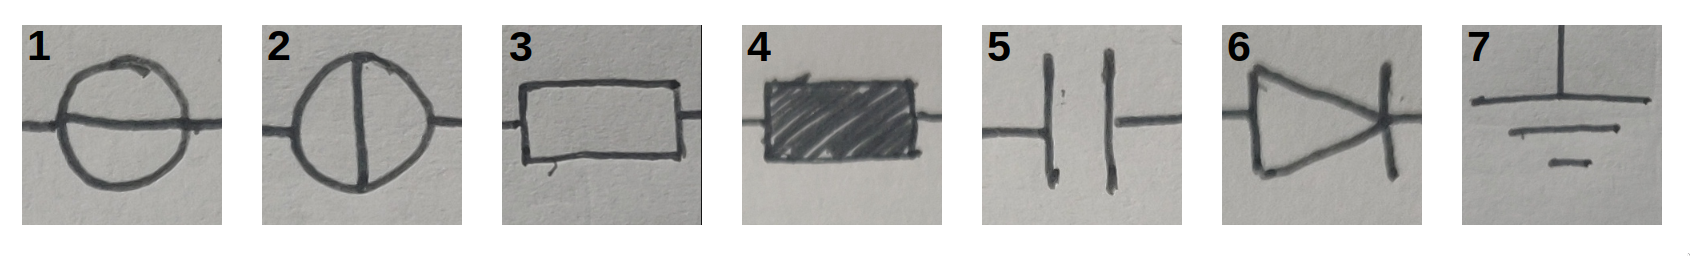
\includegraphics[width=16cm]{imgs/eccs/all.png}
    \caption{All used \acp{ECC} in this thesis in German notation: 1. Voltage Source, 2. Current Source, 3. Resistor, 4. Inductor, 5. Capacitor, 6. Diode, 7. Ground}
    \label{fig:used_eccs}
\end{center}
\end{figure}
